\documentclass[10pt]{article}
\usepackage[margin=1in]{geometry}
\twocolumn
%\usepackage{stfloats} 
\usepackage{graphicx}
\begin{document}
\author{Daniel Speyer\\dls2192@columbia.edu \and Johan Mena\\j.mena@columbia.edu}
\title{A Recursive Systemic Profiler}

\twocolumn[
\begin{@twocolumnfalse}
\maketitle

\end{@twocolumnfalse}
]

\begin{abstract}
The first task in writing any performant code is to understand where it is spending its time. This allows programmers both to apply optimizations where they will make a difference, and to not optimize where it won't make a difference. The standard tools for this are profilers, which measure where processes spend their time while running. However many processes spend most of their total wall time in actions not measured by traditional profilers. Here, we propose and implement a Recursive Systemic Profiler, a tool that can give a more complete view of the causes of an application’s performance in Linux system.
\end{abstract}

\section{Introduction}
Even though premature optimization is the root of all evil, profiling the performance of a system is critical for its improvement. Profiling is, however, no small task: one has to know exactly where in the operating system to look for clues about program behavior, pick the appropriate tool out of several to collect information, and finally make sense of all the data that comes back.

We know from experience that, most of the time, the slowness of systems doesn't come from the entire system as a whole but from very specific parts. As programmers, we want to be able to identify where exactly these parts are so that we can optimize only those parts and not waste time optimizing unimportant parts. We have identified three steps in order to profile programs so they can be optimized: reconnaissance, data collection and data interpretation. We describe each part next.

First, one needs to have an idea about where the slowness of their program is coming from: is the program spending a lot of time doing I/O? Are high levels of concurrency causing lock contention? Does the program depend on an external process to make progress? Depending on the kind of process being analyzed, this can range from being either trivial or hard to identify.

Once one knows where the slowness is coming from, the next step is to collect data. A very typical but rudimentary way to achieve this would be to insert print statements throughout relevant parts of a program. This would allow us to get a sense for how the program would respond, and, to a limited degree, to see if it does what we think it does. However, we all know that this is often not reliable, especially for complex programs that interact with several other pieces. As systems grow and become more complex, it is becoming increasingly important to become familiar with specialized profiling tools that can aid in understanding these kinds of situations.

Finally, once the relevant data has been gathered, one has to interpret it. This is sometimes not as trivial as it sounds because the data could come from many sources: the hardware, the kernel, user applications, etc., and these sources can be, at a high level, seemingly unrelated. However, when data is  presented in different ways, it could tell a different story.

Sample-based tools work by collecting samples of programs at regular intervals.  Samples be performance counters, stack traces, or something else of relevance. These kinds of profilers are typically less accurate than event-based profilers since they rely on, but they since they don't introduce the overhead of generating events, they are usually less intrusive with respect with the profiled application.

The rest of the paper is organized as follows. Section 2 gives an overview of the data collection landscape and kinds of tools profiling tools that are currently available. Section 3 presents BSP's approach to data interpretation through graphs. Section 4 focuses on RSP itself and goes into detail about the concepts it utilizes and the implementation. Section 5 presents evaluations and the results.

\section{Data Collection}
\subsection{Overview}
In order to understand how a system is performing, one first need to collect data. There are several open source profiling tools that focus on this task. We can classify them in three different groups by the approach they use to collect information: event-based, sample-based and a combination of both. 

Event-based tools work by instrumenting programs: they insert marks at different points of a system and trigger an event when the profiled application runs into them. These events can in turn trigger predefined data-collection actions as simple as incrementing counters, but they can also perform more complicated tasks like saving stack dumps for later analysis or generating some kind of logging.

Sample-based tools work by collecting samples of programs at regular intervals.  Samples can come in the form of performance counters, stack traces, or something else of relevance that is already available at the operating system level. These kinds of profilers are typically less accurate than event-based profilers since they rely on samples, but they since they don't introduce the overhead of generating events, they are usually less intrusive with respect with the profiled application.

A third approach combines event-based and sample-based profiling.

\subsection{Current Tools}

There are a variety of open source tools within these categories for collecting data in Linux-based operating systems. They vary in functionality and mode of use depending on, for example, the part of the operating system the user is interested in analyzing or the level of data granularity desired. Some examples of these tools include \begin{tt}perf\end{tt} for system-wide profiling, \begin{tt}strace\end{tt} for system call profiling or \begin{tt}netstat\end{tt} for network profiling.

When we started to ponder ideas for how to gather data to create RSP, one of the first questions that arose was the one about data gathering: could we simply create our custom tool or should we use something that's already available? After researching the profiling landscape for 10 minutes, we found out that data collection was a really challenging task, so we instead decided to piggyback on something proven and reliable. Since RSP focuses on giving users a full-picture view of the system, we decided we needed a tool that provided system-wide reach to gather its data. That tool was \begin{tt}perf\end{tt}.

\subsection{perf}

\begin{tt}perf\end{tt}, also known as \begin{tt}perf\_events\end{tt} and \begin{tt}Linux Perf Events\end{tt}, compared to similar tools like ftrace or lttng, has the advantage of being a mature and actively developed tool that can collect system-wide information in an event-oriented fashion: it is able to tap into hardware events like CPU cycles and memory cache misses; software events like CPU migrations and minor faults; as well as high-level behavior like system calls, TCP events, disk and file system I/O, etc. One can simply choose which kinds of events to track and \begin{tt}perf\end{tt} collects statistics on them. \begin{tt}perf\end{tt} can also filter or log specific system calls. Finally, one of \begin{tt}perf\end{tt}'s more important features as it relates to RSP is the ability to take kernel-space and user-space stacks.

One other characteristic we needed in a tool was the confidence that it was  In addition to these characteristics, perf is part of the Linux kernel itself, so not much extra software is needed in order for one to start profiling applications.

\section{Data Interpretation}
Visualizations are at the heart of the Recursive Systemic Profiler when it comes to interpreting data. Not only do visualizations help to understand what's happening in a system in a shorter period of time compared to looking at plain old numbers, but they also show at-a-glance information that can easily be missed if this is not the case. After evaluating several approaches of data visualization for profilers, we felt the need to emulate the idea of flame graphs.

\subsection{Flame Graphs}
Flame Graphs, a visualization tool invented by Brendan Gregg, are a simple way to visualize profile data through stack traces. Stack traces contain the names of the functions being executed by the CPU at any given time. The information that the stack traces contain can vary depending on the kinds of process being analyzed, the events one requests to be notified of, or the duration of the profiling. Flame graphs present this information in a hierarchical, stack-like manner, in such a way that one can easily tell which stacks of functions were caused by which other stacks of functions, in a pleasant but informative manner.

Flame graphs also have the characteristic of being able to show at a glance overall slow hot-spots (represented by the width of the function calls in the stacks) and overall program structure.


\section{Recursive Systemic Profiler}

The Recursive Systemic Profiler is designed to measure all the activities that contribute to the running time of a program.  It is ``systemic'' in that it records everything that takes place on the system and ``recursive'' in that it starts from a process of interest, then considers processes that was waiting for, and processes those were waiting for, and so on.

The building blocks the profiler works with are runs, sleeps, links and samples.  A run is a contiguous block of time during which a process is running.  A sleep is a similar block in which the process is not running.  A link marks one run causing another.  And a sample is taken by the sampling profiler.  Each sample is part of a run, but very short runs may not have any samples.

\subsection{Scheduling Information}

Linux Perf Events provides annotations for task switches and wakeups, along with stacks.  Task switches are when one process relinquishes a CPU and another takes over (either of the processes may be the idle process).  A stack is given for the departing process.  Wakeups are when a thread becomes marked as runnable (it may not be scheduled for some time).  The Linux kernel is very good at keeping relevant stacks for wakeups.  For example, if a process writes to a TCP socket that connects to localhost, the user function calls write which notices the file handle is a socket and calls send which notices the destination is localhost and calls receive which notices a process is blocked reading from that socket and calls wakeup.  This entire stack is captured intact by perf.

By examining the timing and stacks of these events, we are able to divide task-switches into categories:

\subsection{Interrupts}

Sometimes a process switches out because the CPU it's on has received an interrupt.  Linux uses very small interrupt handlers which pass tasks to high-priority worker threads, rather than do significant work inside the interrupt handler.  This includes cases where a process is pre-empted because it has exhausted its CPU allocation, which we can think of as ``handling a timer interrupt,'' though that is quite rare in practice.

\subsection{Transfers vs Forks}

For non-interrupts, one process wakes another up and then goes to sleep itself.  In this case, we say that one process has ``transfered'' control to another.  When it does not, we say that the thread of control has ``forked''.

\subsection{Pseudo-stacks and Control Paths}

A set of runs connected only by transfer links can be called a ``control path''.

One common pattern is for one process to transfer control to another, and then the other to transfer control back.  Both transfers could be tcp messages, as in the case of making a synchronous rpc request to a database, or one could be a \begin{tt}fork\end{tt} syscall and the other a \begin{tt}wait\end{tt} syscall terminated by the other's exit.  In these cases, it is fairly reasonable to think of the first transfer as a ``function call'' and the second as a ``return''.

While not every pattern of process interaction naturally fits this view, those which don't can generally be shoehorned to fit with fairly little damage.  For example, if one process wakes another which wakes a third which wakes the original, we can think of the first as having been a child of the second, even thought the call went directly.

Once we have this concept of calls and returns, we can assemble the processes into something like a stack.  Note that only the top element of the stack will be a run -- all the rest will be sleeps.

\subsection{Views}

Once we have our data gathered, the next task is to visualize it.  We have several views to do this with.

Our examples here use a toy program called ``pass''.  Pass forks two processes, connects them with pipes, and then runs in a loop in which one process does some work, then writes to one pipe (waking the other process) and reads from the other pipe (blocking on the other process).  It is called ``pass'' because it passes the act of doing work back and forth.

\subsubsection{Process Running View}

The first view is the Process Running View.  It uses an x axis of time and a y axis of processes.  Each run is a block bar, and each link is drawn as a line between them.  The line is red for a transfer, or blue for a fork.

\begin{figure}[h]
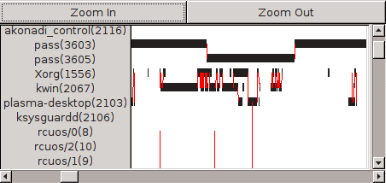
\includegraphics[width=3.25in]{screenshot}
\caption{The Process Running View}
\end{figure}

The view also contains an option to show sleeps, which are drawn as blue boxes.  Sleeps are labeled with one function from the stack which best describes the sleep.  At the moment, this is the innermost userspace function, which roughly corresponds to the blocking syscall as the programmer would conceive of it.

Clicking on a process name opens a Flame View for that process.

\subsubsection{Flame View}

The Flame View takes a single process and shows all associated processes, organized into control paths.  Each control path is treated as a series of pseudostacks, and each layer of each pseudostack is drawn as its stack.  This presents the concept of a single stack of functions stretching across multiple processes, which is a pretty good fit for how many programs are actually designed.

\begin{figure}[h]
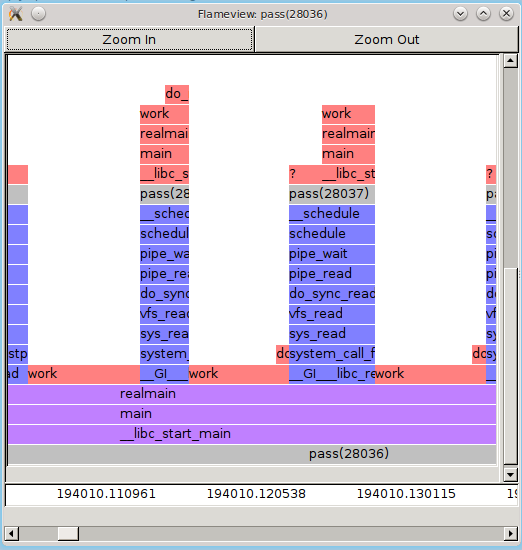
\includegraphics[width=3.25in]{flameshot}
\caption{The Chronological Flame View}
\end{figure}

Functions in a run stack are shown in red, whereas those in a sleep stack are shown in blue.  Process names are shown in grey.  Links are still shown, though links within a control process tend to be largely invisible.

If a run has multiple samples, the horizontal space of the run is divided equally.

The x axis is still time, but now the y axis is stack depth.

\subsection{Implementation}
\subsubsection{Data Collection}

\pretolerance=1000

All data is collected from Linux Perf Events, using \\* the \begin{tt}sched:sched\_wakeup\end{tt}, \begin{tt}sched:sched\_switch\end{tt}, \\* \begin{tt}sched:sched\_process\_exec,\end{tt} \begin{tt}sched:sched\_process\\*\_fork,\end{tt} \begin{tt}block:block\_bio\_queue,\end{tt} and \begin{tt}cycles\end{tt} events.  The data is then dumped in a textual format using the \begin{tt}perf script\end{tt} command.

\pretolerance=200

\subsubsection{Assembling Runs, Sleeps and Links}

The first processing pass simply reads in text and creates a series of event objects.  Each object corresponds to a single event as perf understands the concept.  This pass also attaches stacks to the correct events.

The data is then read into a  state machine that creates runs, sleeps and links.  While passing through, the system keeps track of when each process last started or stopped, what stack each process departed with, and what links are still being assembled.  Links have three timestamps attached: when the wakeup event occurred, when the target process started running, and when the source process stopped running.

Links are created not only from wakeup events, but also from fork and exec.

Links for which the source process stopped less than $100\mu s$ after the wakeup event are regarded as ``transfer'' links.  This number is arbitrary, but seems to work pretty well in practice.

\subsubsection{Working Around Interrupts}

Wakeup events can be identified as interrupts if the departing stack contains either \begin{tt}do\_IRQ\end{tt} or\\ \begin{tt}apic\_timer\_interrupt\end{tt}.  For interrupts, we do not make a link between the processes, but instead make a link between the two runs of the interrupted process that have the interrupt in between them.  This link is marked as ``horizontal'', because it does not correspond to a change of stack layer.

\subsubsection{Recursive Stack Making}

We assemble pseudostacks recursively, going backwards in time.  We start with the process of interest, then look at what woke it and so on.  All wakings are seen as going deeper into the stack unless this would cause a process to appear on the stack twice.  Since a process that is blocked, waiting on the thing it spawned to finish is not listening to other processes, we generally shouldn't one process twice.  There are a few possibilities involving select calls which we will simply accept a suboptimal visualization of, and signals, which are rare.

\subsubsection{Blocking IO}

If a process makes a blocking IO syscall, it will stop, wait for the call to complete, and start again without producing the events discussed thus far.  A process that blocks does create a \begin{tt}block:block\_bio\_queue\end{tt}, but unblocking does not create one (there exists a \begin{tt}block:block\_bio\_complete\end{tt} event, but it doesn't fire in this case, or at least not on our system.  We do, however, see a wakeup event when blocking IOs finish.  The event comes from a swapper thread, but it can be recognized by the function \begin{tt}bio\_endio\end{tt} on its stack.  This does not help us to determine which blocking IO has completed, but we assume it's the same one the thread being woken blocked on.  Once we have this concept of ``a blocking io operation'', we can treat it as a box like a run or a sleep.

\subsubsection{Consolidating}

One thing we have not yet written is a consolidator, that will convert temporal graphs into most-to-least graphs.

\subsubsection{Visualizing}

All visualizations are drawn using gtk.

\section{Evalutation}
\subsection{squirrelmail}

Squirrelmail is a popular, open-source webmail server.  It does not provide its own mail handling, but instead contains an imap client.  Naively, one might think the chain of operations was browser sends tcp to web server forks php interpereter sends tcp to imap server returns data.  In fact, the php interpreter is built into apache (at least in our configuration) and the imap server (dovecot) is rather more complex.  It calls to two other programs: imap and imap-login, the latter of which calls a program called ``auth''.

In fact, auth is where roughly half of the time to produce the webpage is spent.  Of that, one third is spent in computation, mostly sha512, and the rest is spent syncing disks.  The rest of the time is spread about evenly among dovecot, apache and curl.  Very little time remains unaccounted for.

In is unlikely that anyone would guess that most of the time in reading an inbox was spent syncing disk as part of an authentication routine.  Nor can it be easily imagined that any other tool would allow us to discover this.  Furthermore, it seems likely (without looking at auth) that the syncs are unnecessary, and performance could be significantly improved.

A screenshot of the full visualization follows, though it is much more informative with zooming and scrolling than on paper.

\subsection{Other tests}

We plan to run other tests as well, including apt-get, window drag in plasma-desktop and complex webpage rendering.

\newpage

$ $

\newpage

\begin{figure}
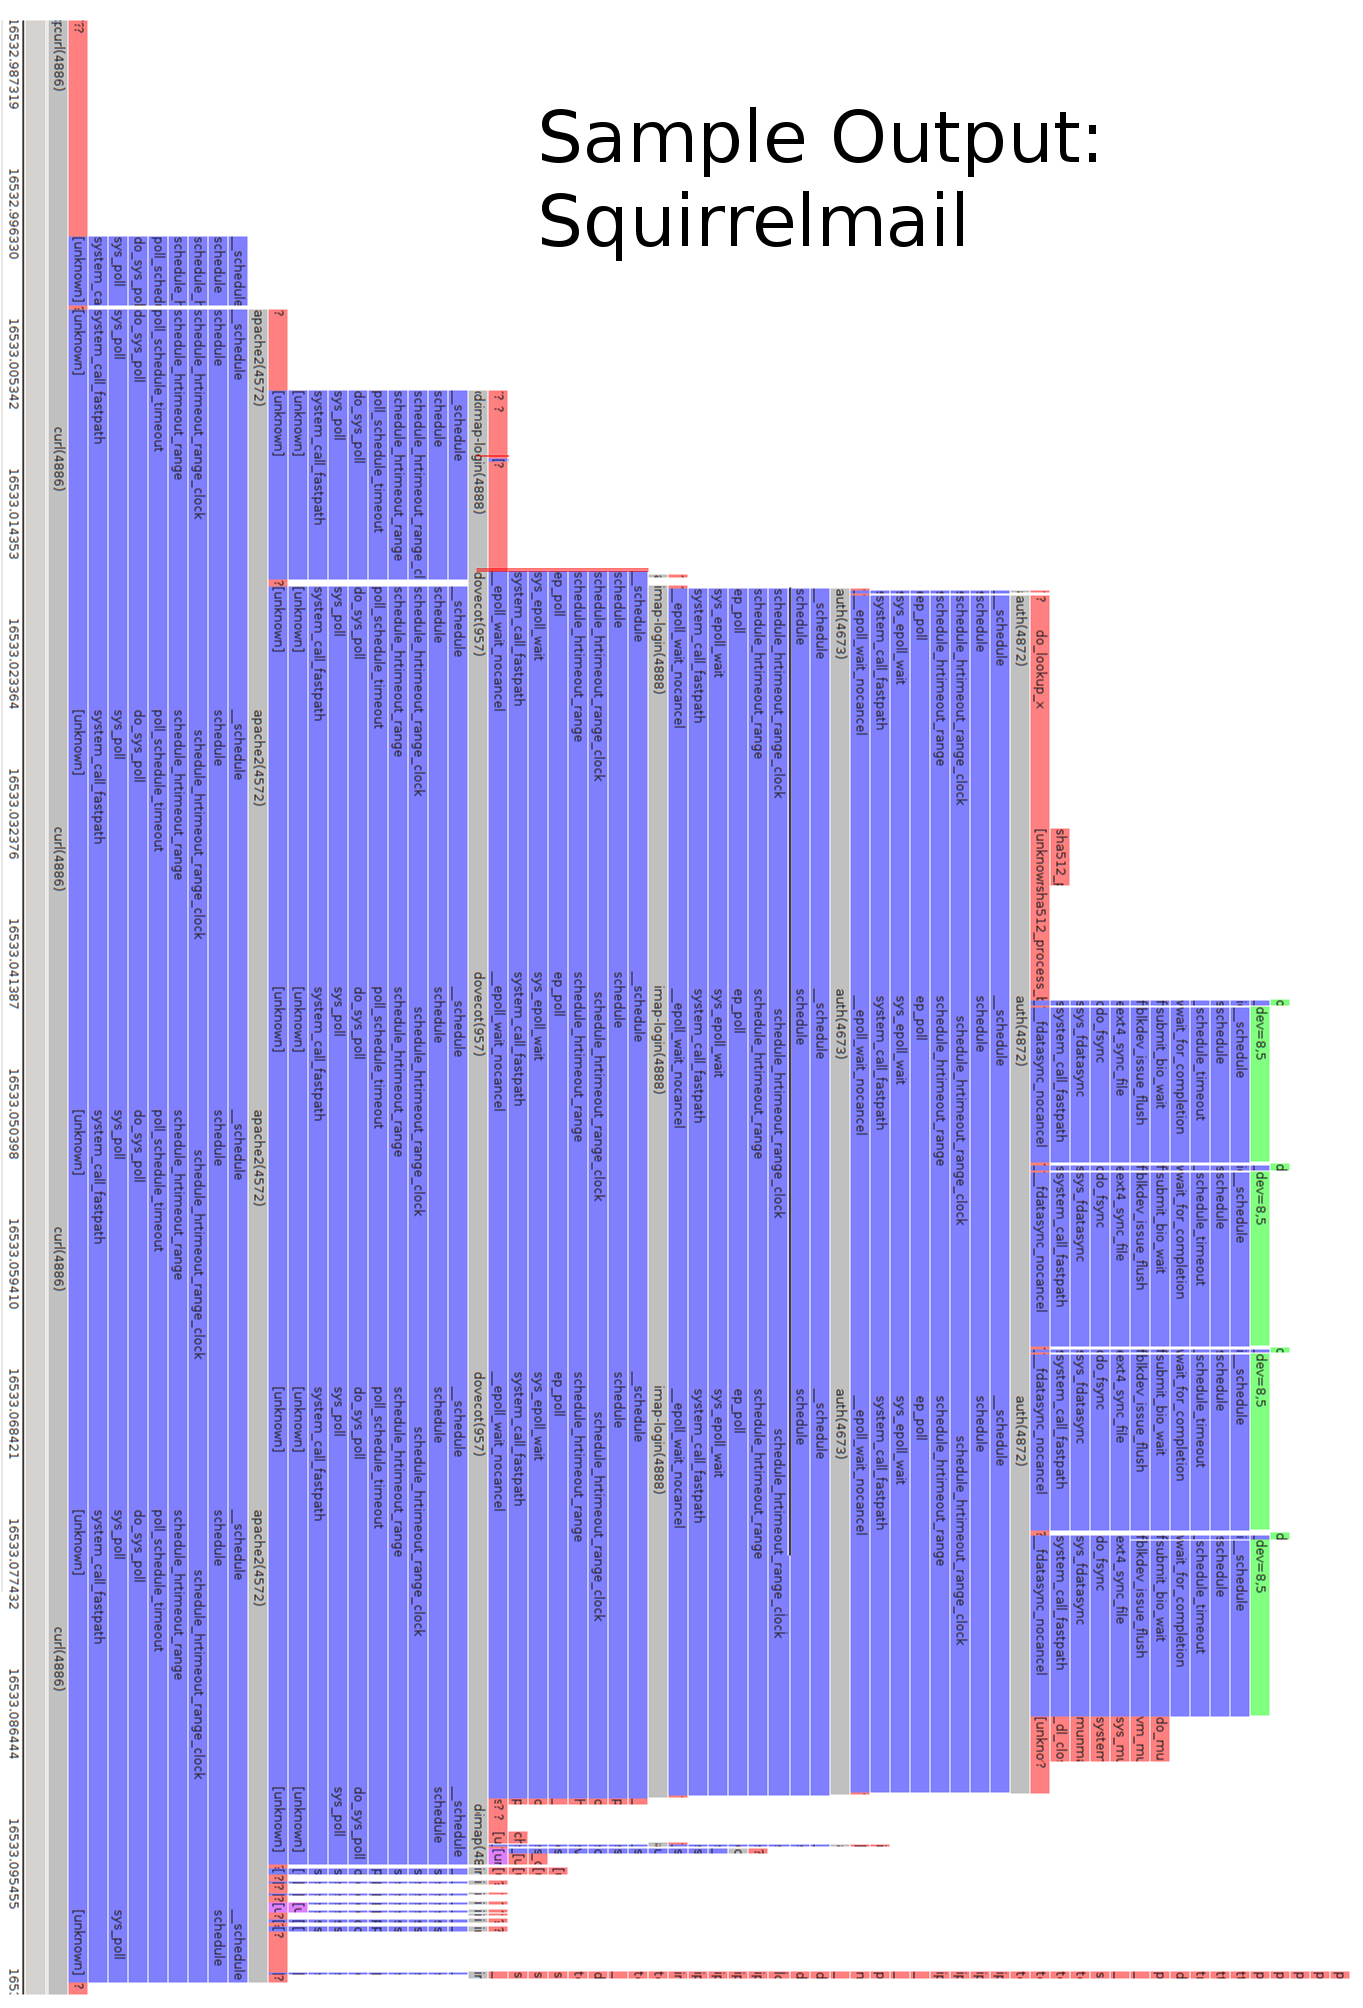
\includegraphics[width=6in]{squirrelmail}
\end{figure}

\end{document}
